%!TEX root =../../../course-notes.tex
% ^ leave for LaTeXTools build functionality


\begin{applicationActivities}



\begin{observation}
Recall that we can model the velocity of a water droplet in a cloud by
\[mv'=-mg-bv\]
where negative numbers represent downward motion,
\(m>0\) is the mass of the droplet, 
\(g>0\) is the magnitude of acceleration due to gravity, and 
\(b>0\) is the proportion of wind resistance to speed.
\begin{center}
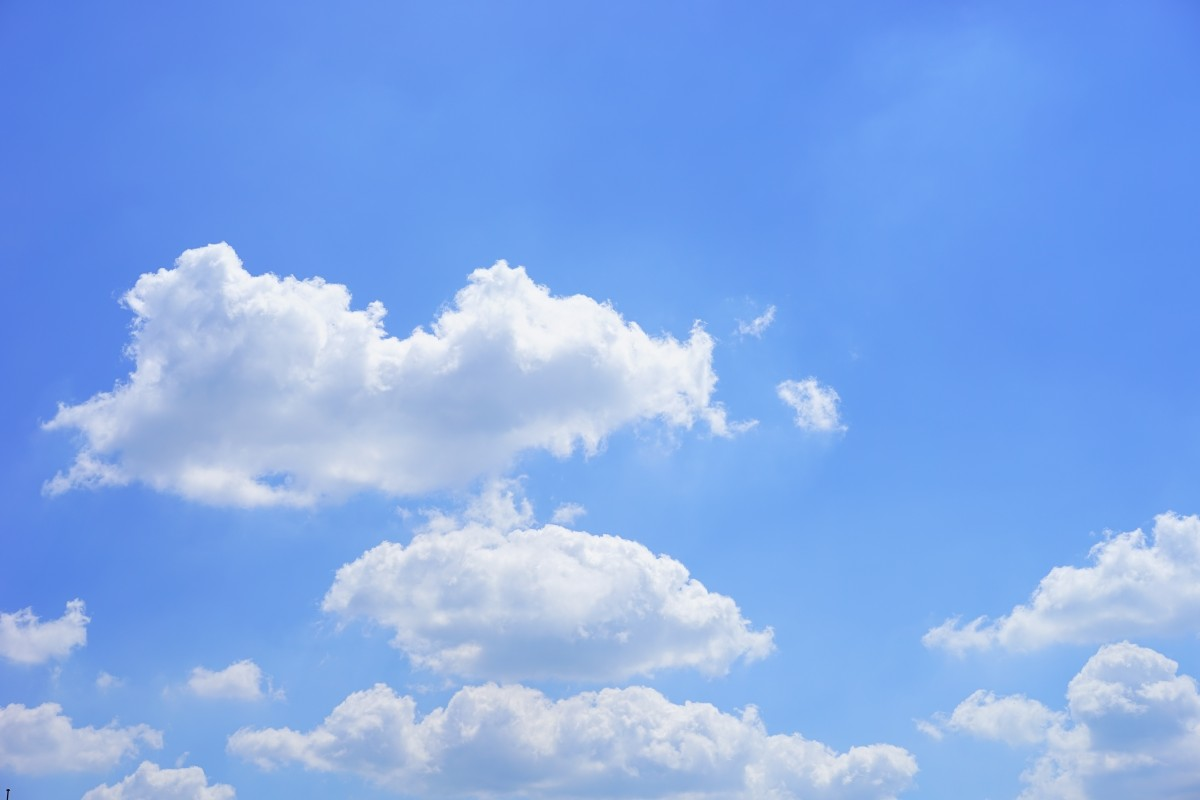
\includegraphics[scale=0.2]{media/cloud.jpg}
\end{center}
\end{observation}

%\begin{activity}{5}
%A water droplet with a radius of \(10\operatorname{\mu m}\) has a mass of about \(4 \times 10^{-15}\operatorname{kg}\).  
%It is determined in a laboratory that for a droplet this size, the constant \(b\) has a value of \(3\times 10^{-3}\operatorname{kg/s}\),
%and it is known that \(g\) is approximately \(9.8\operatorname{m/s}^2\).
%
%\vfill
%
%To study this motion mathematically, which option would you prefer?
%\begin{enumerate}[a)]
%\item Substitute the measurements into the differential equation \(mv'=-mg-bv\) and solve the result:
%\[4\times 10^{-15}v'=-39.2\times 10^{-15}-3\times 10^{-3}v \]
%\item Solve the differential equation in terms of \(m,g,b\) first, and substitute values in later.
%\end{enumerate}
%\end{activity}

\begin{activity}{20}
A water droplet with a radius of \(10\operatorname{\mu m}\) has a mass of about \(4 \times 10^{-15}\operatorname{kg}\).  
It is determined in a laboratory that for a droplet this size, the constant \(b\) has a value of \(3\times 10^{-3}\operatorname{kg/s}\),
and it is known that \(g\) is approximately \(9.8\operatorname{m/s}^2\).

\vfill

Complete the following tasks to study the motion of this droplet.
\begin{subactivity}
Rewrite \(mv'=-mg-bv\) in the form of \(v'+av=\unknown\) for some value of \(a\).
\end{subactivity}
\begin{subactivity}
Find the general solution of this ODE in terms of \(a\) and \(g\). 
(Let \(v_p=wv_0\) when using variation of parameters to avoid confusion.)
\end{subactivity}
\begin{subactivity}
Due to wind resistence, eventually the droplet will effectively stop accelerating upon reaching a certain velocity.
What is this \term{terminal velocity} of the droplet in terms of \(a\) and \(g\)?
\end{subactivity}
\begin{subactivity}
If the droplet starts from rest (\(v=0\) when \(t=0\)), what is its velocity after \(0.01\operatorname{s}\)?
Use a calculator to compute the answer in \(\operatorname{m/s}\).
\end{subactivity}
\end{activity}

\begin{definition}
The last part of the previous activity is an example of an \term{Initial Value Problem (IVP)}; we were given the initial value of the velocity in addition to our differential equation.
\vfill
Physical scenarios often produce IVPs with a unique solution.
\end{definition}

\begin{activity}{10}
Solve the IVP
\[y'+3y=0,\hspace{3em} y(0)=2.\]
\end{activity}

\begin{activity}{10}
Solve the IVP
\[y'-2y=2, \hspace{3em} y(0)=1.\]
\end{activity}

\begin{activity}{5}
Solve the IVP
\[y'-2y=2, \hspace{3em} y(2)=1.\]
\end{activity}


\end{applicationActivities}
